\section{Ecosistema Tecnológico y Perfiles Profesionales}

Para comprender el impacto del aprendizaje automático en el mundo real, es fundamental establecer la diferencia entre las tecnologías que procesan la información y los perfiles humanos responsables de diseñar e implementar estas arquitecturas.

\subsection{1. El Ecosistema Tecnológico (Los Conjuntos)}
Desde un punto de vista matemático y conceptual, la Inteligencia Artificial, el \textit{Machine Learning} y el \textit{Deep Learning} no son disciplinas aisladas, sino subconjuntos anidados donde $DL \subset ML \subset IA$.

\begin{itemize}
    \item \textbf{Inteligencia Artificial (IA):} Es el conjunto universal en este contexto. Abarca cualquier técnica, algoritmo o conjunto de reglas heurísticas que permita a una computadora simular el razonamiento humano. Un sistema de reglas lógicas estrictas clasifica como IA.
    \item \textbf{Aprendizaje Automático (ML):} Es un subconjunto de la IA. Prescinde de las reglas explícitas y emplea estadística computacional y optimización matemática para inducir modelos predictivos a partir de datos históricos.
    \item \textbf{Aprendizaje Profundo (DL):} Es un subconjunto estricto del ML. Se restringe al uso de Redes Neuronales Artificiales de múltiples capas ocultas, especializadas en el aprendizaje automático de representaciones sobre datos no estructurados.
\end{itemize}

\begin{figure}[H]
    \centering
    \shorthandoff{>} % Previene conflictos de Babel
    \resizebox{0.65\textwidth}{!}{%
    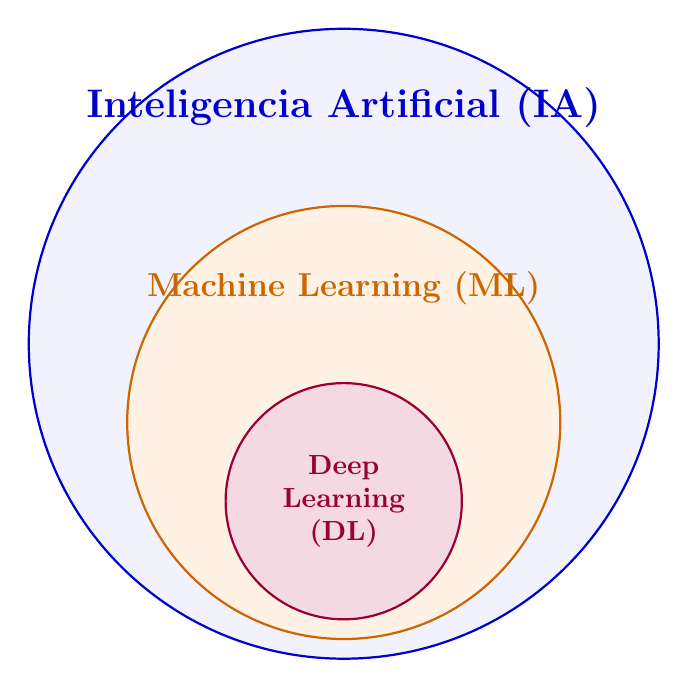
\begin{tikzpicture}[
        font=\sffamily,
        ai/.style={circle, draw=blue!80!black, fill=blue!5, thick, minimum size=8cm},
        ml/.style={circle, draw=orange!80!black, fill=orange!10, thick, minimum size=5.5cm},
        dl/.style={circle, draw=purple!80!black, fill=purple!15, thick, minimum size=3cm}
    ]
    % Conjunto Universal: IA
    \node[ai] (AI) at (0,0) {};
    \node[text=blue!80!black, font=\Large\bfseries, align=center] at (0, 3) {Inteligencia Artificial (IA)};
    % Subconjunto: ML
    \node[ml] (ML) at (0, -1) {};
    \node[text=orange!80!black, font=\large\bfseries, align=center] at (0, 0.7) {Machine Learning (ML)};
    % Subconjunto estricto: DL
    \node[dl] (DL) at (0, -2) {};
    \node[text=purple!80!black, font=\bfseries, align=center] at (0, -2) {Deep\\Learning\\(DL)};
    \end{tikzpicture}%
    }
    \caption{Relación de subconjuntos tecnológicos: El Aprendizaje Profundo es una especialización del Machine Learning, que a su vez es una rama de la Inteligencia Artificial.}
    \label{fig:ai_ml_dl_venn}
\end{figure}

\subsection{2. El Ecosistema de Perfiles (La Cadena de Valor del Dato)}
La implementación de estas tecnologías en entornos productivos requiere una arquitectura robusta operada por tres perfiles fundamentales, los cuales actúan de forma secuencial:

\begin{description}
    \item[A. El Ingeniero de Datos (\textit{Data Engineer}):] Es el arquitecto de la infraestructura subyacente. Se encarga del diseño, construcción y mantenimiento de las canalizaciones (\textit{pipelines}) de datos. Utiliza lenguajes como Python y SQL para ejecutar procesos ETL (Extracción, Transformación y Carga). Su trabajo se despliega frecuentemente en plataformas de computación en la nube, orquestando bases de datos, almacenamiento distribuido y servicios de procesamiento sin servidor para asegurar que los datos estén limpios, integrados y altamente disponibles.
    \item[B. El Analista de Datos (\textit{Data Analyst}):] Actúa en la capa de diagnóstico. Toma los datos estructurados por el ingeniero y aplica estadística descriptiva para inferir el estado actual y pasado de un fenómeno. Su herramienta principal es la visualización de datos mediante tableros interactivos (\textit{dashboards}) que facilitan la toma de decisiones gerenciales.
    \item[C. El Científico de Datos (\textit{Data Scientist}):] Actúa en la capa predictiva y prescriptiva. Su objetivo es modelar la incertidumbre futura aplicando los algoritmos de \textit{Machine Learning} y \textit{Deep Learning} sobre la matriz de datos preparada por el ingeniero. Formula modelos probabilísticos y matemáticos para resolver problemas de regresión, clasificación o agrupamiento.
\end{description}

\subsection{3. Ejemplo Aplicado: Sistema de Inteligencia Turística}
Para ilustrar la sinergia entre estos perfiles, considérese el desarrollo de un Sistema de Inteligencia Turística a escala municipal, cuyo objetivo es gestionar y pronosticar el flujo de visitantes:

\begin{enumerate}
    \item \textbf{Ingeniería de Datos:} El ingeniero desarrolla \textit{scripts} en Python para ingerir datos masivos diarios procedentes de plataformas de alojamiento, sistemas de migración y registros hoteleros. Orquesta estos flujos utilizando infraestructura en la nube (por ejemplo, arquitecturas basadas en \textit{Data Lakes}, catálogos de datos y funciones \textit{Lambda} para procesamiento guiado por eventos), consolidando un repositorio unificado y escalable.
    \item \textbf{Análisis de Datos:} El analista consulta este repositorio mediante SQL para generar un mapa térmico interactivo que revela la densidad histórica de ocupación por zonas geográficas, respondiendo a la pregunta \textit{¿Cómo se distribuyó el turismo el mes pasado?}.
    \item \textbf{Ciencia de Datos:} El científico de datos consume la canalización estructurada por el ingeniero y entrena un modelo predictivo, como una red neuronal recurrente o un ensamble de árboles, para proyectar la tasa de ocupación de las próximas cuatro semanas. Esto permite a la administración pública optimizar dinámicamente los recursos logísticos y de movilidad de la ciudad.
\end{enumerate}